\chapter{Processing your first image}
In this section we'll start with the ``hello world'' app and show you how you can load an image, 
perform some basic processing on the image, draw some stuff on your image and then display your 
results.

Loading images into Java is usually a horrible experience. Using Java \verb+ImageIO+, one can use the 
\verb+read()+ method to create a \verb+BufferedImage+ object. Unfortunately the \verb+BufferedImage+ 
object hides the fact that it is (and in fact all digital raster images are) simply arrays of pixel 
values. A defining philosophy of OpenIMAJ is to \emph{keep things simple} which in turn means in OpenIMAJ 
images are as close as one can get to being \textbf{just arrays of pixel values}.

To read and write images in OpenIMAJ we use the \verb+ImageUtilities+ class. In the \verb+App.java+ 
class file remove the sample code within the main method and add the following line:
\begin{lstlisting}[language=java]
MBFImage image = ImageUtilities.readMBF(
       new File("file.jpg"));
\end{lstlisting}
For this tutorial, read the image from the following URL:
\begin{lstlisting}[language=java]
MBFImage image = ImageUtilities.readMBF(
    new URL("http://dl.dropbox.com/u/8705593/sinaface.jpg"));
\end{lstlisting}
The \verb+ImageUtilities+ class provides the ability to read \verb+MBFImage+s and \verb+FImage+s. 
An \verb+FImage+ is a greyscale image which represents each pixel as a value between \verb+0+ and 
\verb+1+. An \verb+MBFImage+ is a multi-band version of the \verb+FImage+; under the hood it actually
contains a number \verb+FImage+ objects held in a list each representing a band of the image. 
What these bands represent is given by the image's public \verb+colourSpace+ field, which we 
can print as follows:
\begin{lstlisting}[language=java]
System.out.println(image.colourSpace);
\end{lstlisting}
If we run the code, we'll see that the image is an RGB image with three \verb+FImage+s representing 
the red, blue and green components of the image in that order.

You can display any OpenIMAJ image object using the \verb+DisplayUtilities+ class. In this example we display
the image we have loaded then we display the red channel of the image alone: 
\marginpar{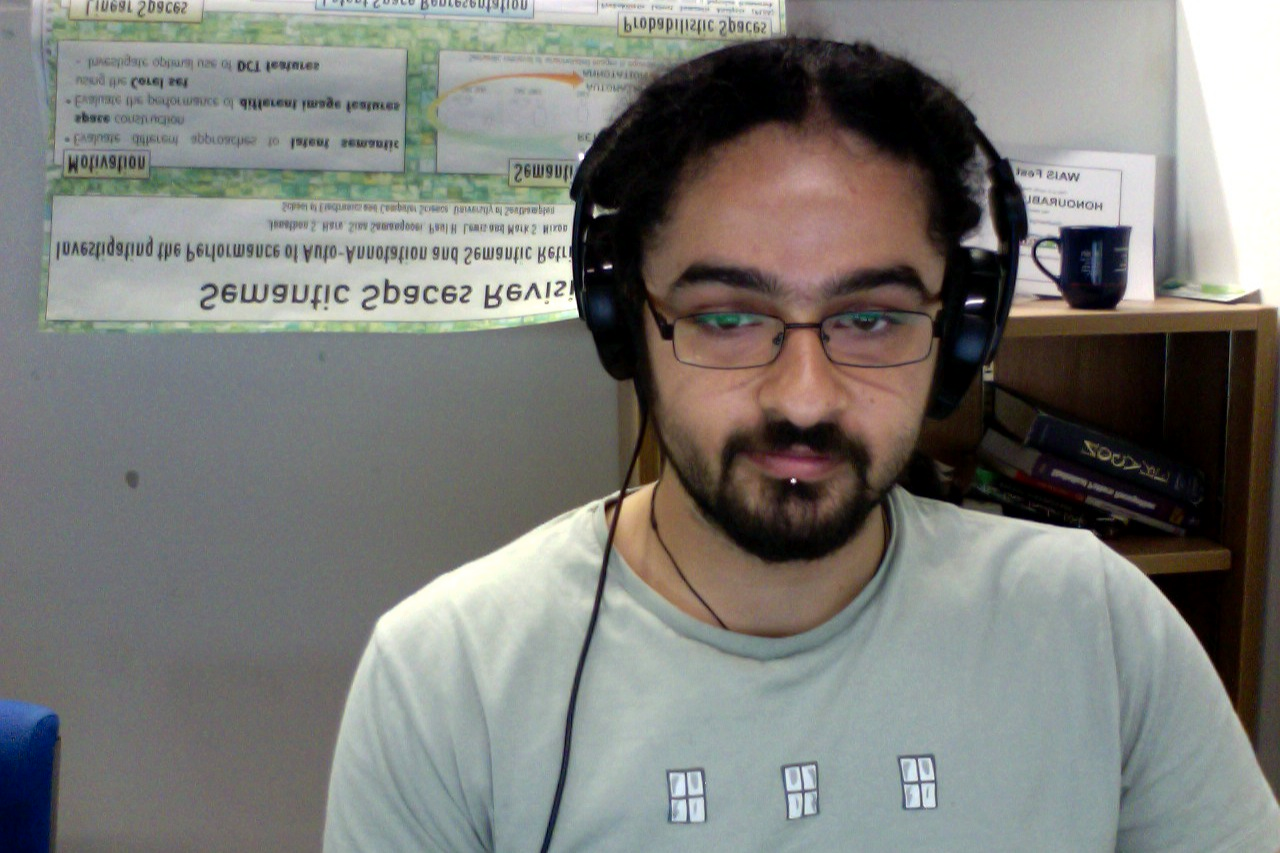
\includegraphics[width=\marginparwidth]{sinaface.png}}
\marginpar{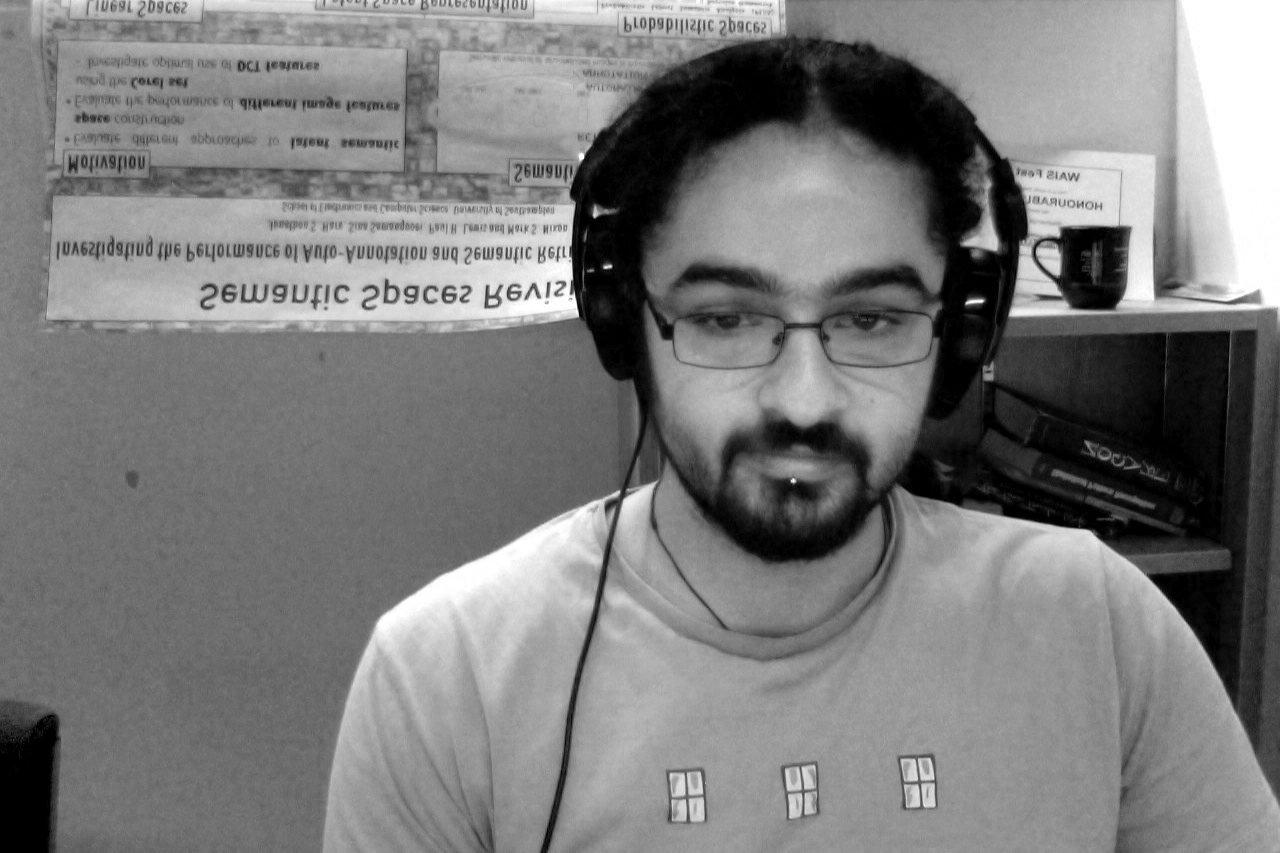
\includegraphics[width=\marginparwidth]{sinaface-rc.png}}
\begin{lstlisting}[language=java]
DisplayUtilities.display(image);
DisplayUtilities.display(
   image.getBand(0), "RedChannel");
\end{lstlisting}

In an image-processing library, images are no good unless you can do something to them. The most basic 
thing you can do to an image is fiddle with its pixels. In OpenIMAJ, as an image is just an array of 
floats, we make this is quite easy. Let's go through our colour image and set all its blue and green 
pixels to black: 
\begin{lstlisting}[language=java]
MBFImage clone = image.clone();
for (int y=0; y<image.getHeight(); y++) {
    for(int x=0; x<image.getWidth(); x++) {
        clone.getBand(1).pixels[y][x] = 0;
        clone.getBand(2).pixels[y][x] = 0;
    }
}
DisplayUtilities.display(clone);
\end{lstlisting}
Note that the first thing we do here is to \verb+clone+ the image to preserve the original image
for the remainder of the tutorial. The pixels in an \verb+FImage+ are held in a 2D float array. The rows 
of the image are held in the first array that, in turn, holds each of the column values for that 
row:  \verb+[y][x]+. By displaying this image we should see an image where two channels are black 
and one channel is not. This results in an image that looks rather red. 
\marginpar{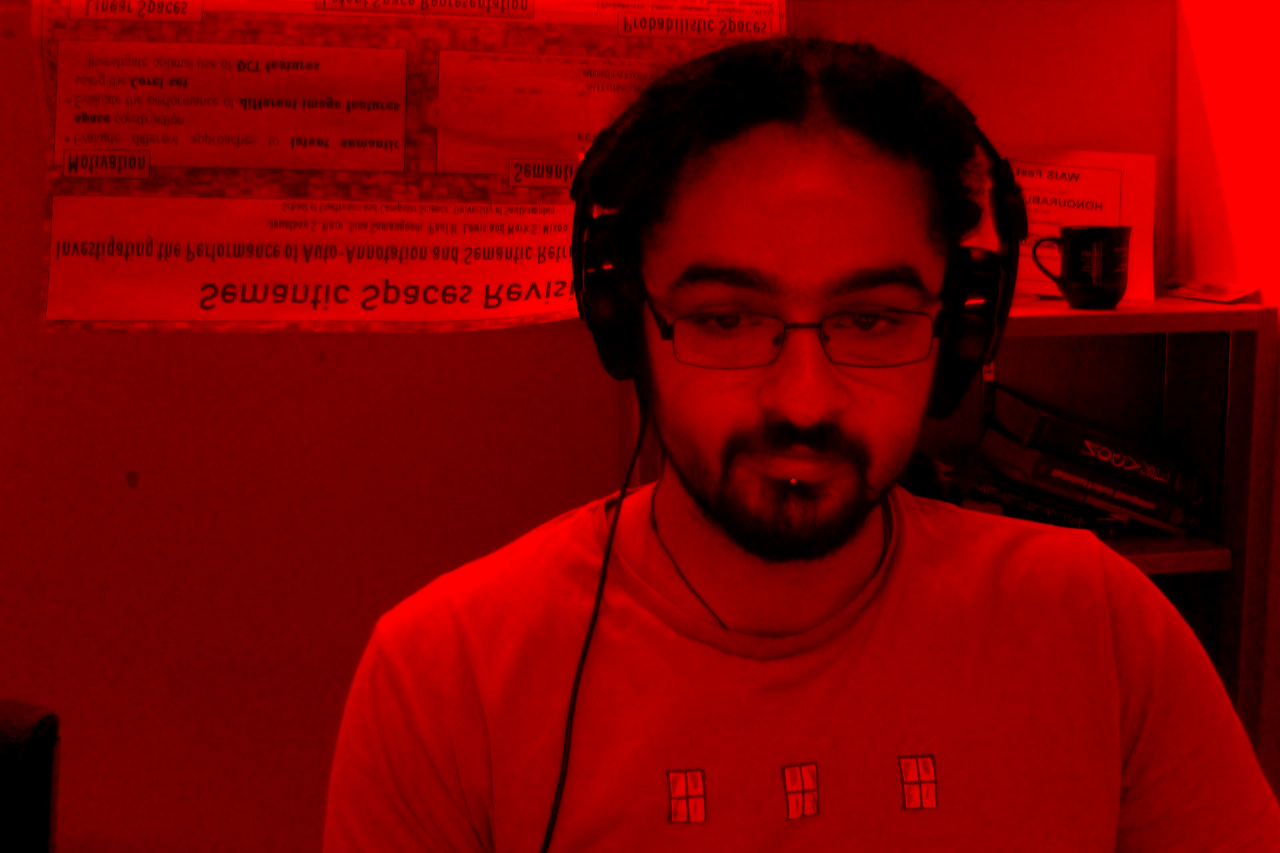
\includegraphics[width=\marginparwidth]{sinaface-red.png}}

Though it is helpful to sometimes get access to individual image pixels, OpenIMAJ provides a lot 
of methods to make things easier. For example, we could have done the above like this instead:
\begin{lstlisting}[language=java]
clone.getBand(1).fill(0f);
clone.getBand(2).fill(0f);
\end{lstlisting}

More complex image operations are wrapped up by OpenIMAJ processor interfaces: \verb+ImageProcessor+s, \verb+KernelProcessor+s,
\verb+PixelProcessor+s and \verb+GridProcessor+s. The distinction between these is how their algorithm works internally. The overarching similarity is that an image goes 
in and a processed image (or data) comes out. For example, a basic operation in image processing 
is \textbf{edge detection}. A popular edge detection algorithm is the \emph{Canny edge detector}. 
We can call the Canny edge detector like so:
\begin{lstlisting}[language=java]
image.processInplace(new CannyEdgeDetector2());
\end{lstlisting}
When applied to a colour image, each pixel of each band is replaced with the edge response at 
that point (for simplicity you can think of this as the difference between that pixel and its 
neighbouring pixels). If a particular edge is only strong in one band or another then that 
colour will be strong, resulting in the psychedelic colours you should see if you display 
the image:
\begin{lstlisting}[language=java]
DisplayUtilities.display(image);
\end{lstlisting}
\marginpar{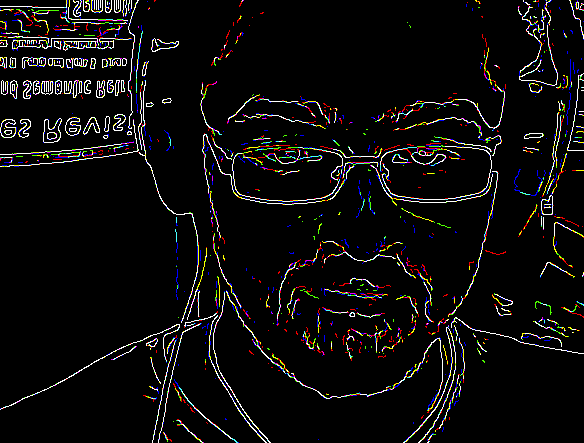
\includegraphics[width=\marginparwidth]{sinaface-canny.png}}

Finally, we can also draw on our image in OpenIMAJ. On every \verb+Image+ object there is a 
set of drawing functions that can be called to draw points, lines, shapes and text on 
images. Let's draw some speech bubbles on our image:
\begin{lstlisting}[language=java]
image.drawShapeFilled(new Ellipse(700f, 450f, 20f, 10f, 0f), RGBColour.WHITE);
image.drawShapeFilled(new Ellipse(650f, 425f, 25f, 12f, 0f), RGBColour.WHITE);
image.drawShapeFilled(new Ellipse(600f, 380f, 30f, 15f, 0f), RGBColour.WHITE);
image.drawShapeFilled(new Ellipse(500f, 300f, 100f, 70f, 0f), RGBColour.WHITE);
image.drawText("OpenIMAJ is", 425, 300, HersheyFont.ASTROLOGY, 20, RGBColour.BLACK);
image.drawText("Awesome", 425, 330, HersheyFont.ASTROLOGY, 20, RGBColour.BLACK);
DisplayUtilities.display(image);
\end{lstlisting}
Here we construct a series of ellipses (defined by their centre [x, y], axes 
[major, minor] and rotation) and draw them as white filled shapes. Finally, we draw 
some text on the image and display it.
\marginpar{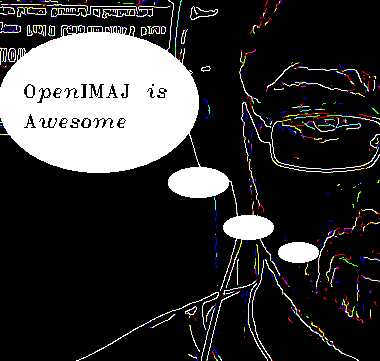
\includegraphics[width=\marginparwidth]{sinaface-awesome.png}}

\section*{Exercises}
\subsection*{Exercise 1: DisplayUtilities}
Opening lots of windows can waste time and space (for example if you wanted to view images on every 
iteration of a process within a loop). In OpenIMAJ we provide a facility to open a 
\emph{named display} so that was can reuse the display referring to it by name. Try to do this with all the 
images we display in this tutorial. Only 1 window should open for the whole tutorial.
\subsection*{Exercise 2: Drawing}
Those speech bubbles look rather plain; why not give them a nice border?
